\documentclass[12pt]{beamer}
\usetheme{Madrid}

\usepackage{amsmath, amsfonts}
\usepackage{hyperref}
\usepackage[super,comma,numbers]{natbib}
\renewcommand{\bibnumfmt}[1]{[#1]}
\bibliographystyle{apsrev4-1}

\title{Diffusion through semi-permeable membranes}
\author[A. Brown]{Aiyan B.}
\date{December 17, 2025}

\newcommand{\abs}[1]{\left| #1 \right|} % | |

\begin{document}

\maketitle

\begin{frame}{Review diffusion model}
    \begin{itemize}
        \item Membrane skeleton (MS) confines the size of cholesterol- and sphingolipid-rich membrane mesodomains, ``rafts''
        \item Idea: 
        slower diffusion in these domains, combined with semi-permeable nature leads to apparent confinement which increase signalling, ``hot-spots''
    \end{itemize}
    \pause
    \begin{figure}
        \centering
        \includegraphics[width=0.7\textwidth]{figures/types-of-diffusion.png}
    \end{figure}
\end{frame}

\begin{frame}{A simple first-approach}
    \begin{columns}
        \begin{column}{0.45\textwidth}
            \begin{figure}
                \centering
                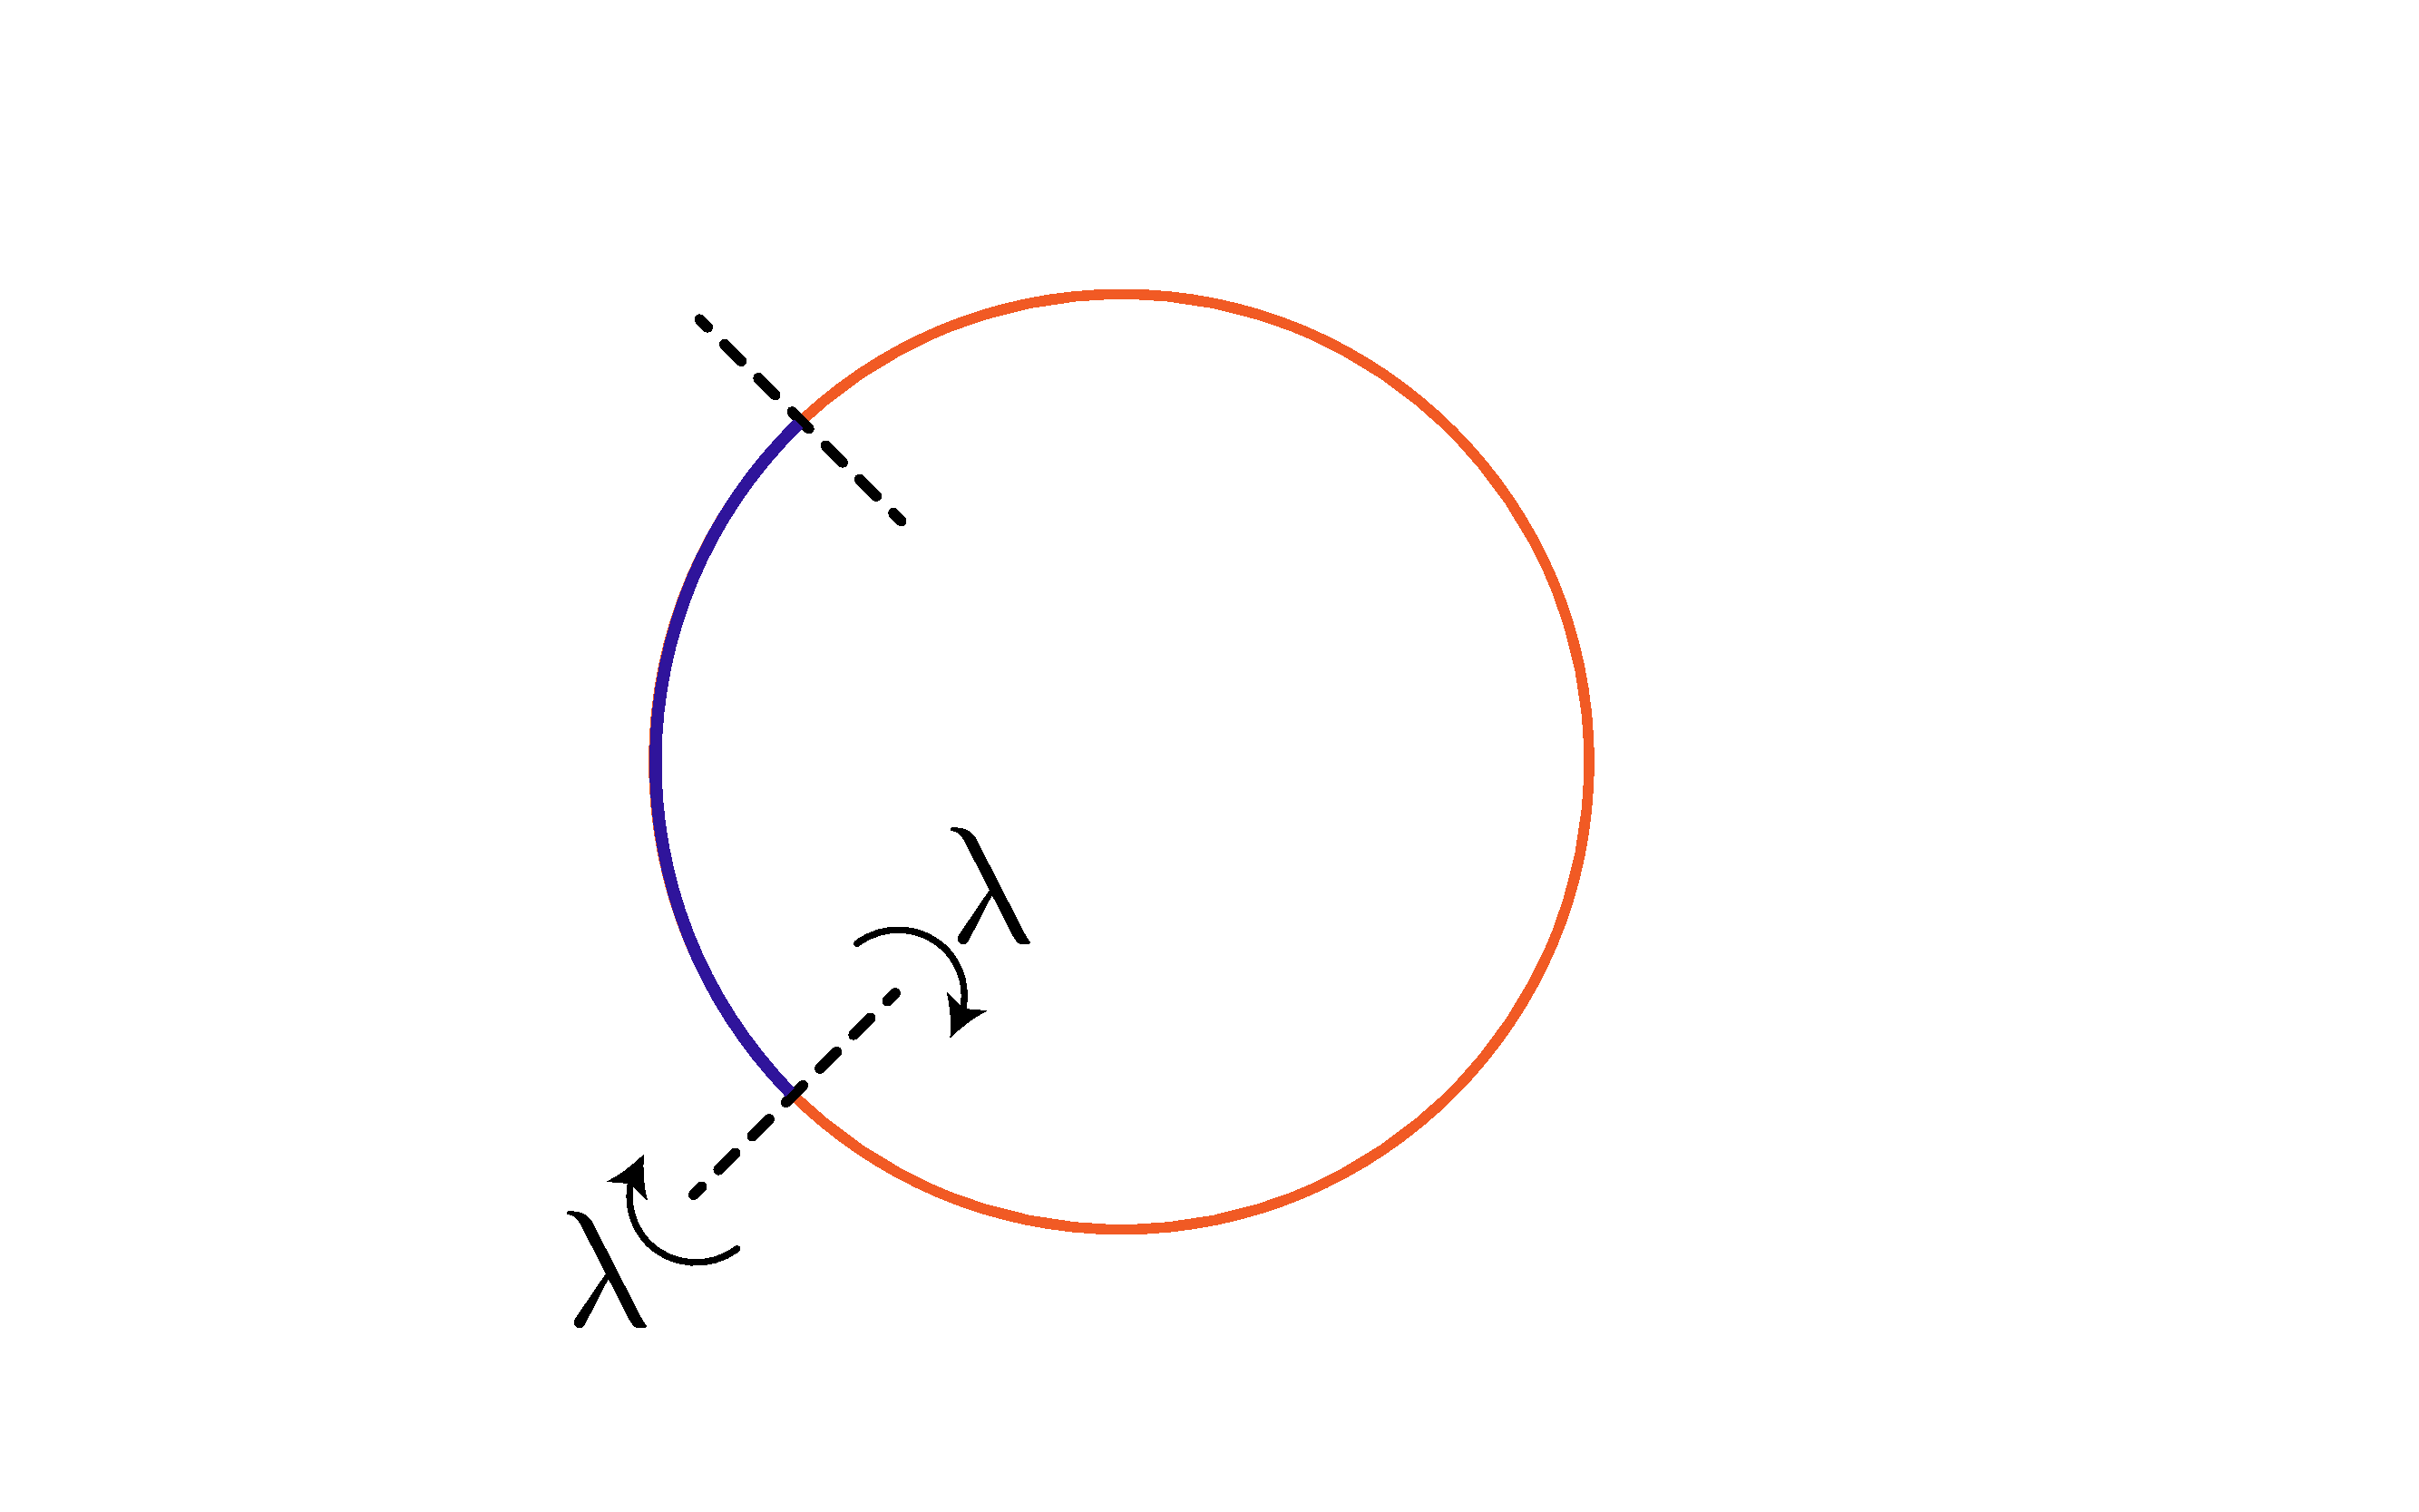
\includegraphics[width=0.925\textwidth]{figures/semi-permeable-model.pdf}
            \end{figure}
        \end{column}
        \begin{column}{0.55\textwidth}
            \begin{enumerate}
                \item Random walk $X_t$ occurs on $\mathbb{Z} \bmod{N}$ where $N$ is the number of lattice sites and $t \in \mathbb{N}$
                \item \textbf{Semi-permeable membranes} are inserted between lattice sites at positions $\{ \mathcal{B}_i \}$
                \pause
                \item Propose a random hopping direction, $X_{t + 1} = X_t \pm 1$
                \item If this move would cross a membrane, $X_t < \mathcal{B}_i$ and $X_{t + 1} > \mathcal{B}_i$ or vice versa, 
                accept with probability $0 < \lambda < 1$, else reflect
            \end{enumerate}
        \end{column}
    \end{columns}
\end{frame}

\begin{frame}{Mean square displacement}
    \begin{itemize}
        \item MSD quickly tapers off to a linear behaviour when integration is performed over a reasonable, $10^{-4}$s, timescale
    \end{itemize}
    \begin{columns}
        \begin{column}{0.5\textwidth}
            \begin{figure}
                \centering
                \includegraphics[width=0.9\textwidth]{figures/trajectory.pdf}
            \end{figure}
        \end{column}
        \begin{column}{0.5\textwidth}
            \begin{figure}
                \centering
                \includegraphics[width=0.9\textwidth]{figures/msd.pdf}
            \end{figure}
        \end{column}
    \end{columns}
\end{frame}

\begin{frame}{Occupation fraction}
    \begin{itemize}
        \item The diffusion coefficient is defined by the fixed quantity $D = a_0^2 / 2 \tau$ where $a_0$ is the lattice spacing and $\tau$ the step size
        \begin{itemize}
            \item Fix $a_0 = 1~\text{nm}$ and let the larger region have diffusivity $D_\mathrm{h} = 1~\mu\text{m}^2/\text{s}$ so $\tau_\mathrm{h} = 0.5~\mu\text{s}$
        \end{itemize}
        \pause
        \begin{columns}
            \begin{column}{0.5\textwidth}
                \begin{figure}
                    \centering
                    \includegraphics[width=0.9\textwidth]{figures/fast-in-barrier.pdf}
                    \caption{%
                        Occupation fraction versus $\lambda \times 10^2$ for $D_\mathrm{l} = 10~\mu\text{m}^2/\text{s}$.
                    }
                \end{figure}
            \end{column}
            \begin{column}{0.5\textwidth}
                \begin{figure}
                    \centering
                    \includegraphics[width=0.9\textwidth]{figures/slow-in-barrier.pdf}
                    \caption{%
                        Occupation fraction versus $\lambda \times 10^2$ for $D_\mathrm{l} = 0.1~\mu\text{m}^2/\text{s}$.
                    }
                \end{figure}
            \end{column}
        \end{columns}
    \end{itemize}
\end{frame}

\begin{frame}{But what about anomalous diffusion?}
    \begin{itemize}
        \item A critical feature of our model is that the ensemble average MSD must have an apparent anomalous behaviour
        \item How can we recover this?
        \begin{enumerate}
            \item Heavy-tailed domain sizes/ diffusivities (quenched radius model~\cite{PhysRevLett.112.150603})
            \pause
            \item Heavy-tailed barrier heights (random barrier model~\cite{PhysRevE.58.4299})
        \end{enumerate}
        \pause
        \item A combination of both might make the most sense: 
        if it is harder for the proteins and raft components to
        escape a given membrane partition (higher barrier height), 
        then we may also expect higher local diffusivity
    \end{itemize}
\end{frame}

\begin{frame}{References}
    \bibliography{references}
\end{frame}

\end{document}